\documentclass[12pt]{article}
% Chinese Support
\usepackage{xeCJK}
\setCJKmainfont{STSong}
% \setmainfont{Times New Roman}

\usepackage{float}

% for symbol
\usepackage{gensymb}
% matrix
\usepackage{amsmath}

% For images
\usepackage{graphicx}
\graphicspath{ {./screenshoot/} }

\newcommand{\numpy}{{\tt numpy}}    % tt font for numpy

\topmargin -1.in
\textheight 9in
\oddsidemargin -.25in
\evensidemargin -.25in
\textwidth 7in


\usepackage{listings}
\usepackage{color}
\usepackage{xcolor}

\definecolor{dkgreen}{rgb}{0,0.6,0}
\definecolor{gray}{rgb}{0.5,0.5,0.5}
\definecolor{mauve}{rgb}{0.58,0,0.82}
\definecolor{textblue}{rgb}{.2,.2,.7}
\definecolor{textred}{rgb}{0.77,0,0}
\definecolor{textgreen}{rgb}{0,0.43,0}

\NeedsTeXFormat{LaTeX2e}[1994/06/01]
\ProvidesPackage{listings-rust}[2018/01/23 Custom Package]

\RequirePackage{color}
\RequirePackage{listings}

\lstdefinelanguage{Rust}{%
  sensitive%
, morecomment=[l]{//}%
, morecomment=[s]{/*}{*/}%
, moredelim=[s][{\itshape\color[rgb]{0,0,0.75}}]{\#[}{]}%
, morestring=[b]{"}%
, alsodigit={}%
, alsoother={}%
, alsoletter={!}%
%
%
% [1] reserve keywords
% [2] traits
% [3] primitive types
% [4] type and value constructors
% [5] identifier
%
, morekeywords={break, continue, else, for, if, in, loop, match, return, while}  % control flow keywords
, morekeywords={as, const, let, move, mut, ref, static}  % in the context of variables
, morekeywords={dyn, enum, fn, impl, Self, self, struct, trait, type, union, use, where}  % in the context of declarations
, morekeywords={crate, extern, mod, pub, super}  % in the context of modularisation
, morekeywords={unsafe}  % markers
, morekeywords={abstract, alignof, become, box, do, final, macro, offsetof, override, priv, proc, pure, sizeof, typeof, unsized, virtual, yield}  % reserved identifiers
%
% grep 'pub trait [A-Za-z][A-Za-z0-9]*' -r . | sed 's/^.*pub trait \([A-Za-z][A-Za-z0-9]*\).*/\1/g' | sort -u | tr '\n' ',' | sed 's/^\(.*\),$/{\1}\n/g' | sed 's/,/, /g'
, morekeywords=[2]{Add, AddAssign, Any, AsciiExt, AsInner, AsInnerMut, AsMut, AsRawFd, AsRawHandle, AsRawSocket, AsRef, Binary, BitAnd, BitAndAssign, Bitor, BitOr, BitOrAssign, BitXor, BitXorAssign, Borrow, BorrowMut, Boxed, BoxPlace, BufRead, BuildHasher, CastInto, CharExt, Clone, CoerceUnsized, CommandExt, Copy, Debug, DecodableFloat, Default, Deref, DerefMut, DirBuilderExt, DirEntryExt, Display, Div, DivAssign, DoubleEndedIterator, DoubleEndedSearcher, Drop, EnvKey, Eq, Error, ExactSizeIterator, ExitStatusExt, Extend, FileExt, FileTypeExt, Float, Fn, FnBox, FnMut, FnOnce, Freeze, From, FromInner, FromIterator, FromRawFd, FromRawHandle, FromRawSocket, FromStr, FullOps, FusedIterator, Generator, Hash, Hasher, Index, IndexMut, InPlace, Int, Into, IntoCow, IntoInner, IntoIterator, IntoRawFd, IntoRawHandle, IntoRawSocket, IsMinusOne, IsZero, Iterator, JoinHandleExt, LargeInt, LowerExp, LowerHex, MetadataExt, Mul, MulAssign, Neg, Not, Octal, OpenOptionsExt, Ord, OsStrExt, OsStringExt, Packet, PartialEq, PartialOrd, Pattern, PermissionsExt, Place, Placer, Pointer, Product, Put, RangeArgument, RawFloat, Read, Rem, RemAssign, Seek, Shl, ShlAssign, Shr, ShrAssign, Sized, SliceConcatExt, SliceExt, SliceIndex, Stats, Step, StrExt, Sub, SubAssign, Sum, Sync, TDynBenchFn, Terminal, Termination, ToOwned, ToSocketAddrs, ToString, Try, TryFrom, TryInto, UnicodeStr, Unsize, UpperExp, UpperHex, WideInt, Write}
, morekeywords=[2]{Send}  % additional traits
%
, morekeywords=[3]{bool, char, f32, f64, i8, i16, i32, i64, isize, str, u8, u16, u32, u64, unit, usize, i128, u128}  % primitive types
%
, morekeywords=[4]{Err, false, None, Ok, Some, true}  % prelude value constructors
% grep 'pub \(type\|struct\|enum\) [A-Za-z][A-Za-z0-9]*' -r . | sed 's/^.*pub \(type\|struct\|enum\) \([A-Za-z][A-Za-z0-9]*\).*/\2/g' | sort -u | tr '\n' ',' | sed 's/^\(.*\),$/{\1}\n/g' | sed 's/,/, /g'    
, morekeywords=[3]{AccessError, Adddf3, AddI128, AddoI128, AddoU128, ADDRESS, ADDRESS64, addrinfo, ADDRINFOA, AddrParseError, Addsf3, AddU128, advice, aiocb, Alignment, AllocErr, AnonPipe, Answer, Arc, Args, ArgsInnerDebug, ArgsOs, Argument, Arguments, ArgumentV1, Ashldi3, Ashlti3, Ashrdi3, Ashrti3, AssertParamIsClone, AssertParamIsCopy, AssertParamIsEq, AssertUnwindSafe, AtomicBool, AtomicPtr, Attr, auxtype, auxv, BackPlace, BacktraceContext, Barrier, BarrierWaitResult, Bencher, BenchMode, BenchSamples, BinaryHeap, BinaryHeapPlace, blkcnt, blkcnt64, blksize, BOOL, boolean, BOOLEAN, BoolTrie, BorrowError, BorrowMutError, Bound, Box, bpf, BTreeMap, BTreeSet, Bucket, BucketState, Buf, BufReader, BufWriter, Builder, BuildHasherDefault, BY, BYTE, Bytes, CannotReallocInPlace, cc, Cell, Chain, CHAR, CharIndices, CharPredicateSearcher, Chars, CharSearcher, CharsError, CharSliceSearcher, CharTryFromError, Child, ChildPipes, ChildStderr, ChildStdin, ChildStdio, ChildStdout, Chunks, ChunksMut, ciovec, clock, clockid, Cloned, cmsgcred, cmsghdr, CodePoint, Color, ColorConfig, Command, CommandEnv, Component, Components, CONDITION, condvar, Condvar, CONSOLE, CONTEXT, Count, Cow, cpu, CRITICAL, CStr, CString, CStringArray, Cursor, Cycle, CycleIter, daddr, DebugList, DebugMap, DebugSet, DebugStruct, DebugTuple, Decimal, Decoded, DecodeUtf16, DecodeUtf16Error, DecodeUtf8, DefaultEnvKey, DefaultHasher, dev, device, Difference, Digit32, DIR, DirBuilder, dircookie, dirent, dirent64, DirEntry, Discriminant, DISPATCHER, Display, Divdf3, Divdi3, Divmoddi4, Divmodsi4, Divsf3, Divsi3, Divti3, dl, Dl, Dlmalloc, Dns, DnsAnswer, DnsQuery, dqblk, Drain, DrainFilter, Dtor, Duration, DwarfReader, DWORD, DWORDLONG, DynamicLibrary, Edge, EHAction, EHContext, Elf32, Elf64, Empty, EmptyBucket, EncodeUtf16, EncodeWide, Entry, EntryPlace, Enumerate, Env, epoll, errno, Error, ErrorKind, EscapeDebug, EscapeDefault, EscapeUnicode, event, Event, eventrwflags, eventtype, ExactChunks, ExactChunksMut, EXCEPTION, Excess, ExchangeHeapSingleton, exit, exitcode, ExitStatus, Failure, fd, fdflags, fdsflags, fdstat, ff, fflags, File, FILE, FileAttr, filedelta, FileDesc, FilePermissions, filesize, filestat, FILETIME, filetype, FileType, Filter, FilterMap, Fixdfdi, Fixdfsi, Fixdfti, Fixsfdi, Fixsfsi, Fixsfti, Fixunsdfdi, Fixunsdfsi, Fixunsdfti, Fixunssfdi, Fixunssfsi, Fixunssfti, Flag, FlatMap, Floatdidf, FLOATING, Floatsidf, Floatsisf, Floattidf, Floattisf, Floatundidf, Floatunsidf, Floatunsisf, Floatuntidf, Floatuntisf, flock, ForceResult, FormatSpec, Formatted, Formatter, Fp, FpCategory, fpos, fpos64, fpreg, fpregset, FPUControlWord, Frame, FromBytesWithNulError, FromUtf16Error, FromUtf8Error, FrontPlace, fsblkcnt, fsfilcnt, fsflags, fsid, fstore, fsword, FullBucket, FullBucketMut, FullDecoded, Fuse, GapThenFull, GeneratorState, gid, glob, glob64, GlobalDlmalloc, greg, group, GROUP, Guard, GUID, Handle, HANDLE, Handler, HashMap, HashSet, Heap, HINSTANCE, HMODULE, hostent, HRESULT, id, idtype, if, ifaddrs, IMAGEHLP, Immut, in, in6, Incoming, Infallible, Initializer, ino, ino64, inode, input, InsertResult, Inspect, Instant, int16, int32, int64, int8, integer, IntermediateBox, Internal, Intersection, intmax, IntoInnerError, IntoIter, IntoStringError, intptr, InvalidSequence, iovec, ip, IpAddr, ipc, Ipv4Addr, ipv6, Ipv6Addr, Ipv6MulticastScope, Iter, IterMut, itimerspec, itimerval, jail, JoinHandle, JoinPathsError, KDHELP64, kevent, kevent64, key, Key, Keys, KV, l4, LARGE, lastlog, launchpad, Layout, Lazy, lconv, Leaf, LeafOrInternal, Lines, LinesAny, LineWriter, linger, linkcount, LinkedList, load, locale, LocalKey, LocalKeyState, Location, lock, LockResult, loff, LONG, lookup, lookupflags, LookupHost, LPBOOL, LPBY, LPBYTE, LPCSTR, LPCVOID, LPCWSTR, LPDWORD, LPFILETIME, LPHANDLE, LPOVERLAPPED, LPPROCESS, LPPROGRESS, LPSECURITY, LPSTARTUPINFO, LPSTR, LPVOID, LPWCH, LPWIN32, LPWSADATA, LPWSAPROTOCOL, LPWSTR, Lshrdi3, Lshrti3, lwpid, M128A, mach, major, Map, mcontext, Metadata, Metric, MetricMap, mflags, minor, mmsghdr, Moddi3, mode, Modsi3, Modti3, MonitorMsg, MOUNT, mprot, mq, mqd, msflags, msghdr, msginfo, msglen, msgqnum, msqid, Muldf3, Mulodi4, Mulosi4, Muloti4, Mulsf3, Multi3, Mut, Mutex, MutexGuard, MyCollection, n16, NamePadding, NativeLibBoilerplate, nfds, nl, nlink, NodeRef, NoneError, NonNull, NonZero, nthreads, NulError, OccupiedEntry, off, off64, oflags, Once, OnceState, OpenOptions, Option, Options, OptRes, Ordering, OsStr, OsString, Output, OVERLAPPED, Owned, Packet, PanicInfo, Param, ParseBoolError, ParseCharError, ParseError, ParseFloatError, ParseIntError, ParseResult, Part, passwd, Path, PathBuf, PCONDITION, PCONSOLE, Peekable, PeekMut, Permissions, PhantomData, pid, Pipes, PlaceBack, PlaceFront, PLARGE, PoisonError, pollfd, PopResult, port, Position, Powidf2, Powisf2, Prefix, PrefixComponent, PrintFormat, proc, Process, PROCESS, processentry, protoent, PSRWLOCK, pthread, ptr, ptrdiff, PVECTORED, Queue, radvisory, RandomState, Range, RangeFrom, RangeFull, RangeInclusive, RangeMut, RangeTo, RangeToInclusive, RawBucket, RawFd, RawHandle, RawPthread, RawSocket, RawTable, RawVec, Rc, ReadDir, Receiver, recv, RecvError, RecvTimeoutError, ReentrantMutex, ReentrantMutexGuard, Ref, RefCell, RefMut, REPARSE, Repeat, Result, Rev, Reverse, riflags, rights, rlim, rlim64, rlimit, rlimit64, roflags, Root, RSplit, RSplitMut, RSplitN, RSplitNMut, RUNTIME, rusage, RwLock, RWLock, RwLockReadGuard, RwLockWriteGuard, sa, SafeHash, Scan, sched, scope, sdflags, SearchResult, SearchStep, SECURITY, SeekFrom, segment, Select, SelectionResult, sem, sembuf, send, Sender, SendError, servent, sf, Shared, shmatt, shmid, ShortReader, ShouldPanic, Shutdown, siflags, sigaction, SigAction, sigevent, sighandler, siginfo, Sign, signal, signalfd, SignalToken, sigset, sigval, Sink, SipHasher, SipHasher13, SipHasher24, size, SIZE, Skip, SkipWhile, Slice, SmallBoolTrie, sockaddr, SOCKADDR, sockcred, Socket, SOCKET, SocketAddr, SocketAddrV4, SocketAddrV6, socklen, speed, Splice, Split, SplitMut, SplitN, SplitNMut, SplitPaths, SplitWhitespace, spwd, SRWLOCK, ssize, stack, STACKFRAME64, StartResult, STARTUPINFO, stat, Stat, stat64, statfs, statfs64, StaticKey, statvfs, StatVfs, statvfs64, Stderr, StderrLock, StderrTerminal, Stdin, StdinLock, Stdio, StdioPipes, Stdout, StdoutLock, StdoutTerminal, StepBy, String, StripPrefixError, StrSearcher, subclockflags, Subdf3, SubI128, SuboI128, SuboU128, subrwflags, subscription, Subsf3, SubU128, Summary, suseconds, SYMBOL, SYMBOLIC, SymmetricDifference, SyncSender, sysinfo, System, SystemTime, SystemTimeError, Take, TakeWhile, tcb, tcflag, TcpListener, TcpStream, TempDir, TermInfo, TerminfoTerminal, termios, termios2, TestDesc, TestDescAndFn, TestEvent, TestFn, TestName, TestOpts, TestResult, Thread, threadattr, threadentry, ThreadId, tid, time, time64, timespec, TimeSpec, timestamp, timeval, timeval32, timezone, tm, tms, ToLowercase, ToUppercase, TraitObject, TryFromIntError, TryFromSliceError, TryIter, TryLockError, TryLockResult, TryRecvError, TrySendError, TypeId, U64x2, ucontext, ucred, Udivdi3, Udivmoddi4, Udivmodsi4, Udivmodti4, Udivsi3, Udivti3, UdpSocket, uid, UINT, uint16, uint32, uint64, uint8, uintmax, uintptr, ulflags, ULONG, ULONGLONG, Umoddi3, Umodsi3, Umodti3, UnicodeVersion, Union, Unique, UnixDatagram, UnixListener, UnixStream, Unpacked, UnsafeCell, UNWIND, UpgradeResult, useconds, user, userdata, USHORT, Utf16Encoder, Utf8Error, Utf8Lossy, Utf8LossyChunk, Utf8LossyChunksIter, utimbuf, utmp, utmpx, utsname, uuid, VacantEntry, Values, ValuesMut, VarError, Variables, Vars, VarsOs, Vec, VecDeque, vm, Void, WaitTimeoutResult, WaitToken, wchar, WCHAR, Weak, whence, WIN32, WinConsole, Windows, WindowsEnvKey, winsize, WORD, Wrapping, wrlen, WSADATA, WSAPROTOCOL, WSAPROTOCOLCHAIN, Wtf8, Wtf8Buf, Wtf8CodePoints, xsw, xucred, Zip, zx}
%
, morekeywords=[5]{assert!, assert_eq!, assert_ne!, cfg!, column!, compile_error!, concat!, concat_idents!, debug_assert!, debug_assert_eq!, debug_assert_ne!, env!, eprint!, eprintln!, file!, format!, format_args!, include!, include_bytes!, include_str!, line!, module_path!, option_env!, panic!, print!, println!, select!, stringify!, thread_local!, try!, unimplemented!, unreachable!, vec!, write!, writeln!}  % prelude macros
}%

\lstdefinestyle{colouredRust}%
{ basicstyle=\ttfamily%
, identifierstyle=%
, commentstyle=\color[gray]{0.4}%
, stringstyle=\color[rgb]{0, 0, 0.5}%
, keywordstyle=\bfseries% reserved keywords
, keywordstyle=[2]\color[rgb]{0.75, 0, 0}% traits
, keywordstyle=[3]\color[rgb]{0, 0.5, 0}% primitive types
, keywordstyle=[4]\color[rgb]{0, 0.5, 0}% type and value constructors
, keywordstyle=[5]\color[rgb]{0, 0, 0.75}% macros
, columns=spaceflexible%
, keepspaces=true%
, showspaces=false%
, showtabs=false%
, showstringspaces=true%
}%

\lstdefinestyle{boxed}{
  style=colouredRust%
, numbers=left%
, firstnumber=auto%
, numberblanklines=true%
, frame=trbL%
, numberstyle=\tiny%
, frame=leftline%
, numbersep=7pt%
, framesep=5pt%
, framerule=10pt%
, xleftmargin=15pt%
, backgroundcolor=\color[gray]{0.97}%
, rulecolor=\color[gray]{0.90}%
}

% \setmonofont{FiraCode-Regular}
\lstset{frame=tb,
  language=Rust,
  aboveskip=3mm,
  belowskip=3mm,
  showstringspaces=false,
  columns=flexible,
  basicstyle={\ttfamily},
  numbers=none,
  numberstyle=\tiny\color{gray},
  keywordstyle=\color{blue}\itshape,
  stringstyle=\color{mauve},
  breaklines=true,
  breakatwhitespace=true,
  commentstyle=\color{textred}\itshape,
  tabsize=3
}
\usepackage{indentfirst}
\usepackage{bm}
\usepackage[ruled]{algorithm2e}
\usepackage{cite}

% Content start below
\begin{document}

\author{陈铭涛\\16340024}
\title{数据挖掘第二次项目\\
    \large{并行决策树集成}}
% \date{\vspace{-5ex}}
\maketitle

\medskip

% ========== Begin answering questions here

\section{CART 算法}

决策树是一种树结构,每一个非叶子节点表示一个对一个特征的分裂,叶子节点存放了分类问题中的类别和回归问题中的数值。
其对样本进行预测的方法是从根节点开始,根据每一个分支节点的特征属性,决定输出方向直到到达叶子节点,将叶子节点的数值作为输出值。

决策树的优点为决策过程较为容易令人理解,可解释性强。决策树的构造方法包括了 ID3, C4.5等算法,在本次项目中主要实现的是 CART 算法。

CART 包含了分类决策树和回归决策树的算法,本次实现了其中的回归树算法。CART 构造出的决策树为一棵二叉树。对于分类问题,CART 算法通过 Gini Index 来计算数据集的纯度,以决定一个节点的分裂,其公式如下:

假设样本集合$D$中第$k$类样本比例为$p_k$($k=1,2...|N|$),
\begin{equation}
    \begin{aligned}
    Gini(D)=1-\sum_{k=1}^{|N|}p_k^2
    \end{aligned}
\end{equation}

$Gini(D)$反映了从$D$中随机抽取两个样本其类别不同的概率,越小则代表样本纯度越高。对于属性集合$A$上的属性$a$,将所有$D$上取值为$a^v$的样本记为$D^v$,则$a$上的Gini Index为:
\begin{equation}
    Gini(D, a)=\sum_{v=1}^{|V|}\frac{|D^v|}{|D|}Gini(D^v)
\end{equation}
选择$A$中的划分点即为
\begin{equation}
    a_*=\mathop{\arg\min}_{a\in A}Gini(D,a)
\end{equation}

当要解决的问题是回归问题时,假设样本集合$D$中第$i$个样本的标签为$y_i$,则最小化的目标为回归标签的平方误差和,即
\begin{equation}
    SSE(D)=\sum_{i=1}^{|N|}(y_i-\overline{y})^2
\end{equation}

对于在属性$a$上的$v$值分裂的节点,设其左子树和右子树上的样本集合分别为$D^L$, $D^R$, 则其平方误差和为:
\begin{equation}
    SSE(D, a, v)=SSE(D^L) + SSE(D^R)
\end{equation}

则对于属性$a$上的划分点的选择为:
\begin{equation}
    a_*=\mathop{\arg\min}_{a\in A, v \in V}SSE(D,a,v)
\end{equation}

CART 算法进行决策树构建的方法如下:

\begin{algorithm}[H]
    \SetAlgoLined
    \KwResult{分类决策树或回归决策树 }
    从深度为0开始构建\;
    对各连续特征列进行排序\;

    \While{未达到终止条件}{
        \uIf{特征为连续特征}{
            从排序好的特征列中对每一个取值进行评判标准的计算\;
            选取令评判标准最小的取值作为分裂点\;
        }
        \uElseIf{特征为类别特征}{
            从样本中选取令评判标准最小的类别进行分裂\;
        }
        根据分裂点创建新的决策树节点
    }
    \caption{CART 决策树构建}
\end{algorithm}

其中的终止条件如下:
\begin{enumerate}
    \item 若节点中的所有样本的标签值均相同
    \item 若树的深度已达到用户定义的\lstinline{MaxDepth}数值
    \item 若节点的样本数少于用户定义的\lstinline{MinSamplesSplit}数值
    \item 若节点的分裂生成的子节点样本数少于用户定义的\lstinline{MinSamplesLeaf}数值
\end{enumerate}

在实现中,由于本次项目的数据特征均为连续特征,只实现了在连续特征下的回归决策树构建。

由于对于连续变量的特征,$|V|$可能是一个较大的数值,此时对连续变量的每一个不同值进行扫描的计算代价非常大,因此实现中添加了\lstinline{MaxBin}参数,在寻找分裂点时程序将会将特征列分为对应的段数,每段仅测试一个分裂点。将该参数调大可以提升训练结果,但是会增加训练时间。

\section{并行化实现}
在决策树训练过程中可选的实现并行化的位置为\cite{fang_2015}:
\begin{enumerate}
    \item 并行化进行对每一层节点的分裂
    \item 每个节点的分裂中对每个特征进行并行化处理
    \item 在每一层中对每个特征进行并行化处理
\end{enumerate}

在实现的代码中,选择的是在训练一层的过程中对各节点与特征进行并行化处理,每个节点上测试完所有特征的分裂可能后根据评判标准选择最优的分裂点进行分裂。

\section{Gradient Boosting}

Gradient Boosting 是一种结合多个弱学习器的集成方法,每一步中训练的模型尝试去“纠正”先前输出的模型。

设训练集为$\{(x_i, y_i)\}_{i=1}^n$, 模型预测值$\hat{y}=F(x)$, 学习率 $\alpha$,使用的可微分损失函数为均方误差:
\begin{equation}
    \begin{aligned}
    L(y, \hat{y}) = \frac{1}{N}\sum_{i=1}^{n}(y_i - \hat{y_i})^2\\
    \end{aligned}
\end{equation}

对损失函数除2后求偏导数得到:
\begin{equation}
    \frac{\partial L(y, F(x))}{\partial F(x)}=F(x)-y
\end{equation}

即模型输出与标签的残差取负数。由梯度下降算法的思想可知延残差方向移动可降低损失函数。由此可得当损失函数为均方误差时 Gradient Boosting 中每步的模型更新方法。

综上,令算法迭代次数为$M$, Gradient Boosting 算法如下:

\begin{algorithm}[H]
    \SetAlgoLined
    \KwResult{ 模型 $F_M(x)$ }
    初始化$F_0(x)=\mathop{\arg\min}_{\gamma} L(y, \gamma)$\;
    

    \For{$m=1$ to $M$}{
        \begin{enumerate}
            \item 计算残差数值:
            \begin{equation}
                r_{m}=-\left[\frac{\partial L(y, F_{m-1}(x))}{\partial F_{m-1}(x)}\right] = y-F_{m-1}(x)
            \end{equation}
            \item 以 $\{(x, r_{m})\}$ 作为训练集训练一个弱学习模型(此处为决策树)$h_m(x)$
            \item 更新模型$F_m(x)=F_{m-1}(x)+\alpha h_m(x)$
        \end{enumerate}
    }
    \caption{Gradient Boosting}
\end{algorithm}

在代码实现中,每次迭代增加了对学习率的从0至1的线性搜索,从而不使用固定的学习率,而是在每一步中找到令当前步最优的学习率:
\begin{equation}
    \alpha_m = \mathop{\arg\min}_\alpha L(y, F_{m-1}(x)+\alpha h_m(x))
\end{equation}

学习率搜索过程可以并行进行,使用这种方法可以在较少迭代次数下较固定学习率获得更好的成绩,在迭代数较大的时候分数可能不如固定较小的学习率。

由以上算法说明可知 Gradient Boosting 整体是串行运行的,因此在 Gradient Boosting 算法中只能对基学习器即决策树的训练部分进行并行的实现。


\section{Random Forest}

Random Forest 采用 Bagging 的方法进行决策树集成。Bagging 集成的算法如下:

输入训练集$(X, Y)$,训练轮数$M$,采样大小$n$, 基学习器训练算法$H$

对于训练集有放回采样获得$M$个大小为$n$的训练集$\{(X_i, Y_i)\}_{i=1}^M$

\begin{algorithm}[H]
    \SetAlgoLined
    \KwResult{ 模型 $F(x)$ }
    
    \For{$m=1$ to $M$}{
        $h_m = H(X_m, Y_m)$
    }
    对于分类问题,采用投票法获得最终模型,对于回归问题,采用取平均方法获得最终模型\;
    \caption{Bagging}
\end{algorithm}

随机森林算法则在 Bagging 算法的基础上增加了随机属性选择,即在决策树中的每个节点,先从属性集合中选出一个大小为$k$的子集,再从该子集中选择划分点进行分裂。$k$的取值决定了模型的随机程度。

随机森林中通过加入属性扰动来对只有样本扰动的 Bagging 集成方法进行改进,使得最终集成泛化性因为个体学习器之间的差异性增加而增加。

由随机森林的算法可知,不同的基学习器之间是可以并行进行训练的,但是由于在实现中已经对决策树实现了并行训练,若对基学习器也并行化只会增加上下文切换的开销,因此没有实现基学习器的并行训练。

\section{代码实现}

出于内存、速度和并行化实现的考虑,本次项目选择了使用 Rust 语言实现,原因是 Rust 的 RAII 机制使得资源可以及时地释放,提升内存利用率;由编译器提供的静态检查可以避免多线程时线程不安全的情况,降低 debug 难度;作为通过 LLVM 后端编译为机器代码的静态语言 Rust 可以在相同的实现下获得比 Python 等语言更高的速度。使用的编译器版本为\lstinline{rustc 1.35.0}.

程序实现中使用的第三方库如下:
\begin{enumerate}
    \item rayon: 提供基于迭代器的便捷地编写并行代码的方法
    \item rand: 提供随机数生成
    \item csv: 提供对 csv 文件的读取
    \item indicatif: 提供命令行进度条实现
    \item ndarray: 提供类似 numpy 的多维数组的操作
    \item num-traits: 提供数值类型上的一些实用方法,如最大最小值等
    \item log: 程序日志
    \item pretty\_env\_logger: 程序日志输出
    \item num\_cpus: 获取系统 CPU 核心数量
    \item serde: 提供将结构体变量序列化的功能
    \item serde\_json: 用于以 json 格式将序列化后的模型变量保存至文件
\end{enumerate}

项目中包括的主要代码文件如下
\begin{enumerate}
    \item[$\bullet$] data\_frame.rs: 使用一个二维的 \lstinline{ndarray} 作为程序使用的 \lstinline{DataFrame} 类型,并定义了类型别名\lstinline{V} 作为全局的数据存储类型,可设为 \lstinline{f64} 或 \lstinline{f32}, 此外还包含了 csv 文件读写等其他实用函数
    \item[$\bullet$] learner.rs: 定义了一个学习器 \lstinline{Learner} trait,包括了类似于 sklearn 的\lstinline{fit} 和\lstinline{predict} 两个方法,决策树,Boosting和 Random Forest 都需实现该 trait。
    \item[$\bullet$] tree.rs: 包括了 \lstinline{DecisionTree}类型,实现了 CART 算法,可对单个决策树进行训练和预测。
    \item[$\bullet$] boosting.rs: 包括了\lstinline{GradientBoosting} 类型的定义与训练和预测的实现。
    \item[$\bullet$] random\_forest.rs: 包括了\lstinline{RandomForest} 类型的定义与训练和预测的实现。
    \item[$\bullet$] utils 目录:包括了数个实用功能,如获取数据列排序序列,交叉验证,模型分数计算等。
\end{enumerate}

bin 目录下的包含 main 函数的可执行代码文件如下:
\begin{enumerate}
    \item[$\bullet$] boost\_cv.rs:使用 GDBT 进行交叉验证
    \item[$\bullet$] boost\_predict.rs:使用 GDBT 进行训练并输出在测试集上的预测结果
    \item[$\bullet$] cv.rs:使用单棵决策树进行交叉验证
    \item[$\bullet$] parallel\_performance.rs:接收一个命令行整数作为程序最多使用的线程数,进行一次单棵决策树的训练,用于测试并行化的效率
    \item[$\bullet$] predict.rs:使用单棵决策树进行训练并输出测试集预测结果
    \item[$\bullet$] rf\_cv.rs:使用随机森林进行交叉验证
    \item[$\bullet$] rf\_predict.rs:使用随机森林进行训练并输出测试集预测结果
\end{enumerate}

调参的方式为在 bin 目录下的可执行代码文件中找到\lstinline{tree_config} 和 \lstinline{boost_config} 或\lstinline{forest_config} 并修改对应参数字段的数值。

程序运行前需将训练数据放置在项目上层目录下的 data 文件夹下。

运行任一 bin 目录下的代码的方法为在项目目录下执行命令(*nix系统下),其中\lstinline{EMTM_LOG=info}的作用是使程序将日志输出到命令行:
\begin{lstlisting}
EMTM_LOG=info cargo run --release --bin {EXEC_NAME}
\end{lstlisting}

所有代码都需在 release 模式下进行编译,否则速度可能会有20到100倍的减慢。


\section{并行化表现}

由于并行化的实现主要位于单棵决策树的训练中,对于并行化表现的测试主要针对单棵决策树的训练与预测。

在命令行下使用如下命令测试了从单线程到12线程下对单棵决策树训练时的时间:
\begin{lstlisting}
for ((i = 1; i<=12;i++)) cargo run --release --bin parallel_performance $i >>../threads_performance.txt
\end{lstlisting}

将获得的训练速度相对单线程下训练速度的提升数据进行绘图如下:
\begin{figure}[H]
    \centering
    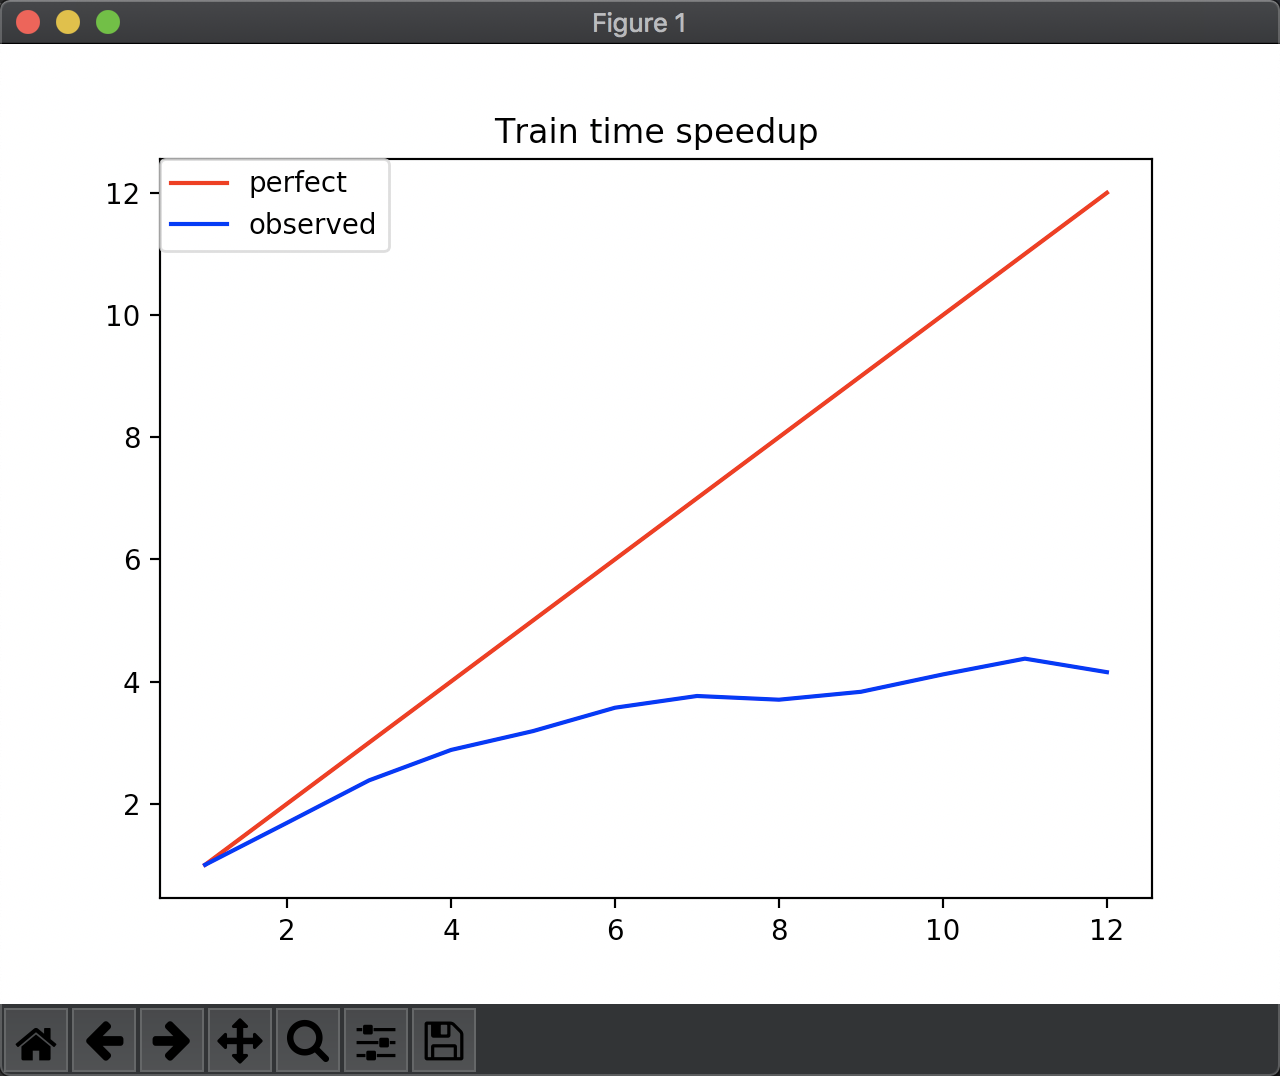
\includegraphics[scale=0.4]{train_time_speedup.png}
    \caption{并行训练速度提升情况}
    \label{}
\end{figure}

预测速度的数据进行绘图如下:
\begin{figure}[H]
    \centering
    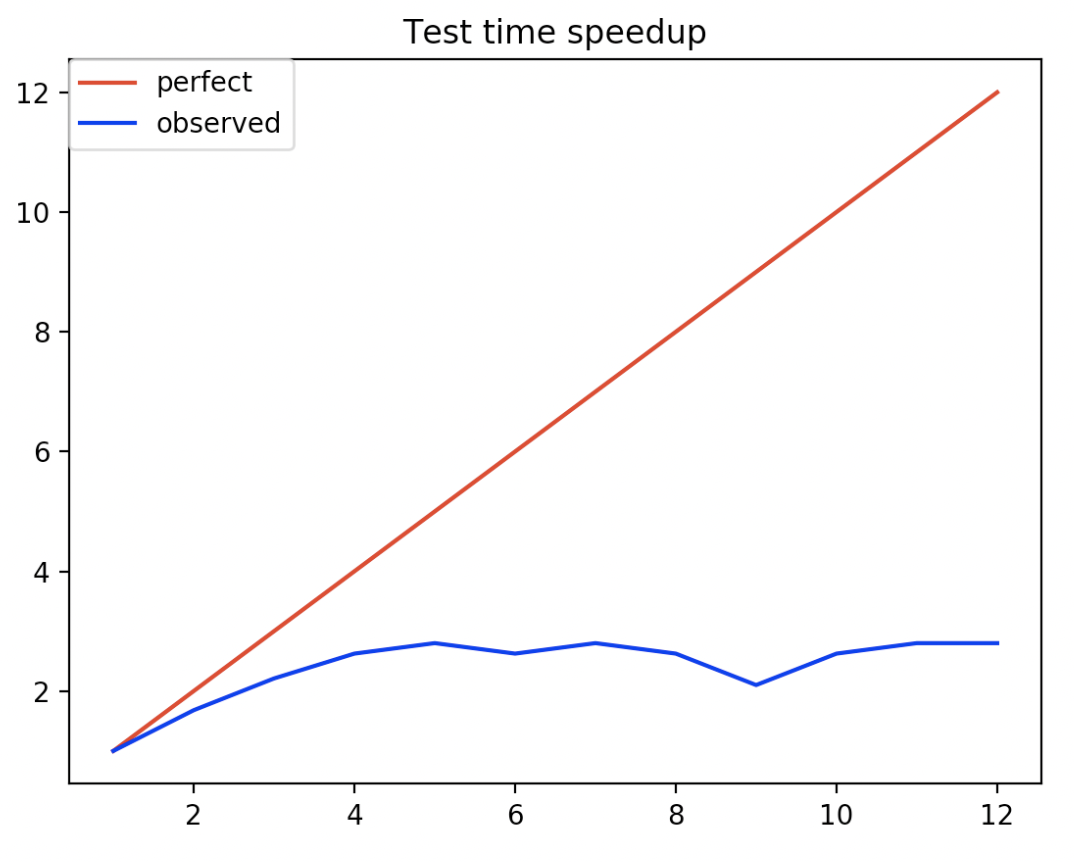
\includegraphics[scale=0.4]{test_time_speedup.png}
    \caption{并行预测速度提升情况}
    \label{}
\end{figure}

可见当线程数提升到一定程度下对训练速度的提升大约收敛在 4 倍,而对预测速度的提升不大。

\section{验证}
以下程序测试均在一台搭载6核12线程 CPU,运行 macOS 系统的笔记本电脑上运行,数据精度为\lstinline{f64}。
\\

验证的标准为$R^2$, 其计算方法如下:

\begin{equation}
    \begin{aligned}
    \bar{y}= \frac{1}{n}\sum_{i=1}^n y_i,\\
    SS_{tot} = \sum_i(y_i-\overline{y})^2,\\
    SS_{res} = \sum_i(y_i-f_i)^2,\\
    R^2 = 1 - \frac{SS_{res}}{SS_{tot}}
    \end{aligned}
\end{equation}

其中$y_i$为第$i$个样本的实际观察值,$f_i$为第$i$个样本的模型预测值。$R^2$的取值通常在0与1之间,越接近1代表预测值与真实值匹配程度越高。


使用 \lstinline{LightGBM} \cite{NIPS2017_6907} 构建一个模型运行3折交叉验证进行对比:

\begin{figure}[H]
    \centering
    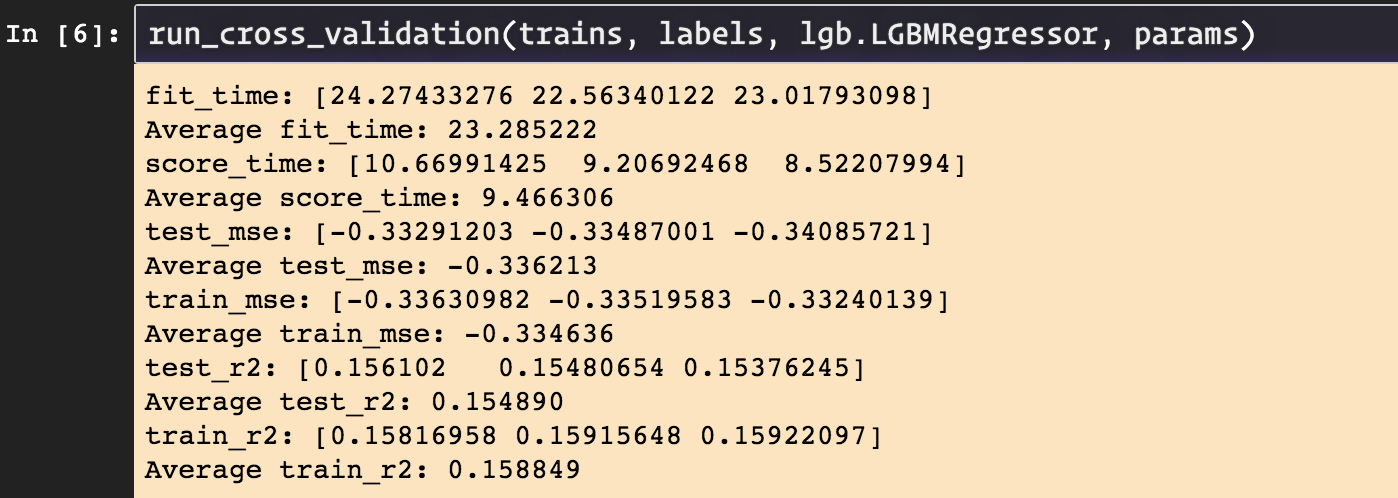
\includegraphics[scale=0.6]{lgb-baseline.png}
    \caption{LightGBM 交叉验证结果}
    \label{}
\end{figure}

对单棵决策树进行交叉验证获得的结果如下:

在训练集上获得的平均$R^2$分数为0.14947528261278345

在验证集上获得的平均$R^2$分数为0.143995380629807

训练时间平均为 682423 ms.

\begin{figure}[H]
    \centering
    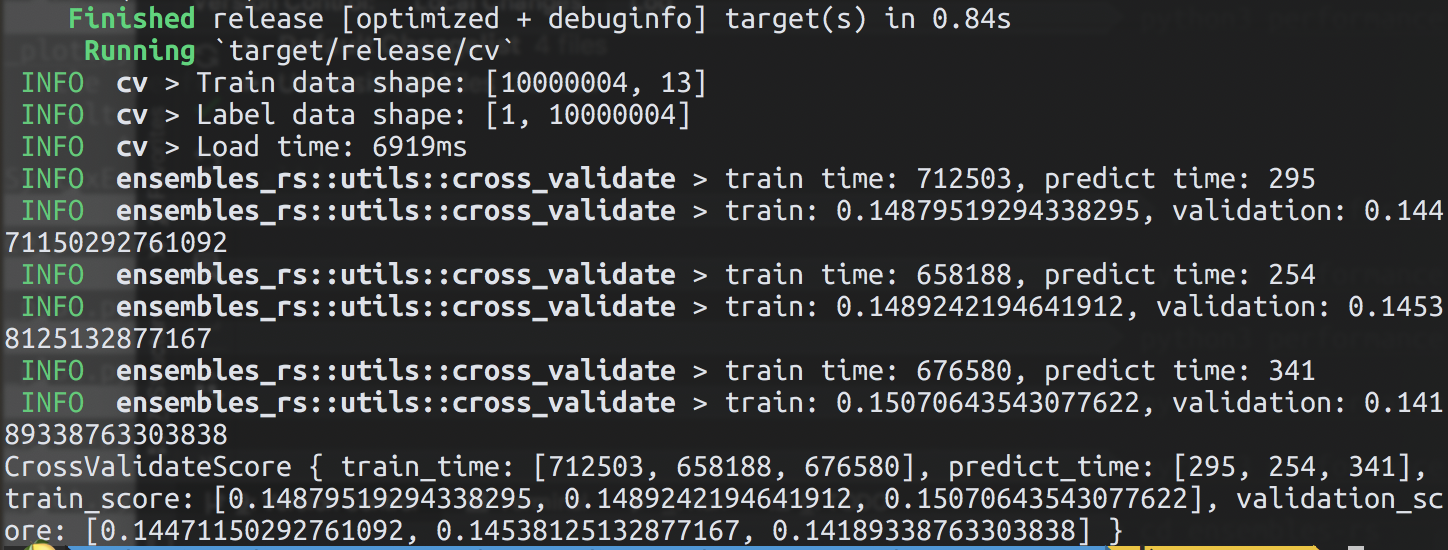
\includegraphics[scale=0.6]{single-tree-cv.png}
    \caption{单棵决策树训练交叉验证结果}
    \label{}
\end{figure}

使用 Gradient Boosting 训练150步,设置单棵树最大生长至 2 层,进行交叉验证获得的结果如下:

在训练集上获得的平均$R^2$分数为0.14595633826167811

在验证集上获得的平均$R^2$分数为0.14329480642795986

训练时间平均为 223031 ms.

\begin{figure}[H]
    \centering
    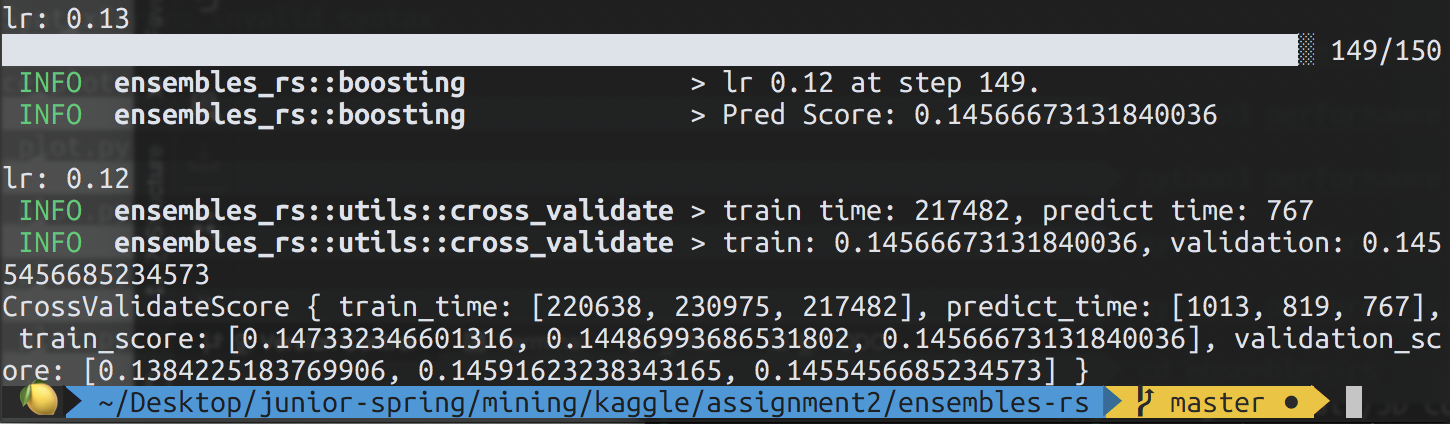
\includegraphics[scale=0.6]{gbdt-cv.png}
    \caption{GBDT 训练交叉验证结果}
    \label{}
\end{figure}

使用 Random Forest 训练,决策树数量为150,不限制决策树生长深度,进行交叉验证获得的结果如下:

在训练集上获得的平均$R^2$分数为0.15712251333333332

在验证集上获得的平均$R^2$分数为0.15363599666666664

训练时间平均为 1355728 ms.

\begin{figure}[H]
    \centering
    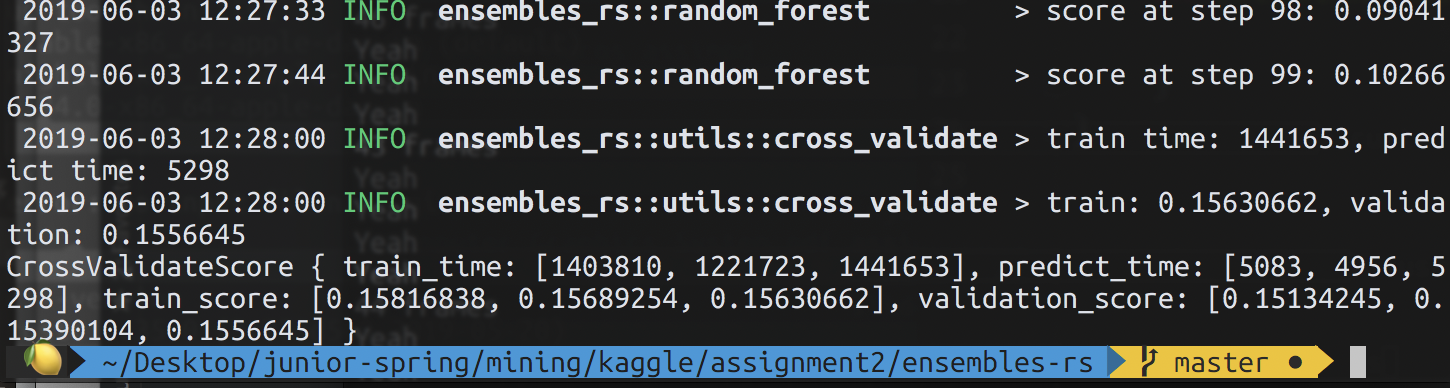
\includegraphics[scale=0.6]{rf-cv.png}
    \caption{随机森林训练交叉验证结果}
    \label{}
\end{figure}

四个训练中使用取样工具查看内存占用峰值分别如下:
\begin{enumerate}
    \item LightGBM: 5.2G
    \begin{figure}[H]
        \centering
        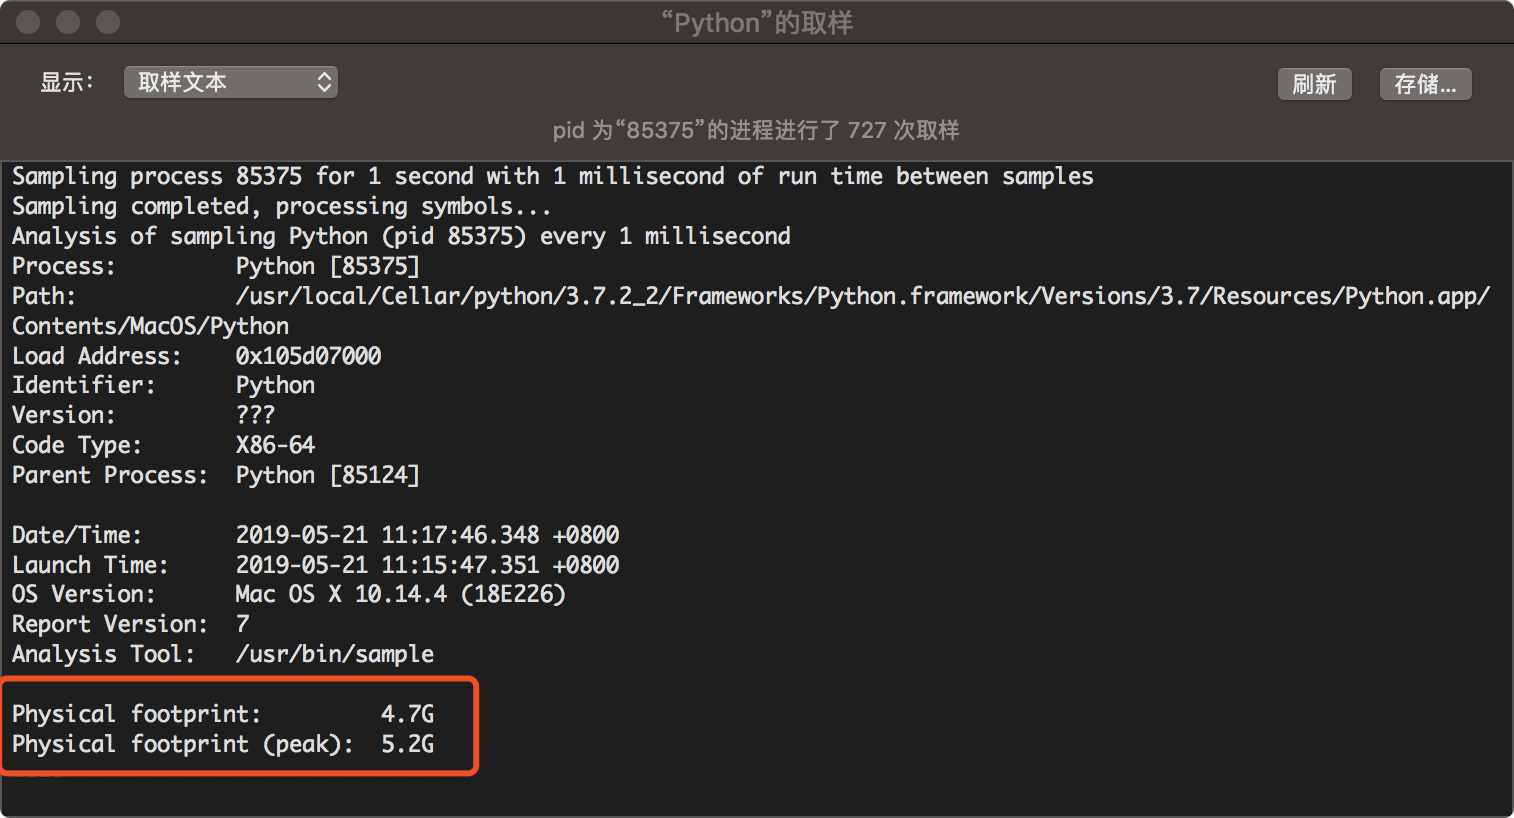
\includegraphics[scale=0.46]{lgb-memory.png}
        \caption{LightGBM 内存占用}
        \label{}
    \end{figure}

    \item 单决策树:3.2G
    \begin{figure}[H]
        \centering
        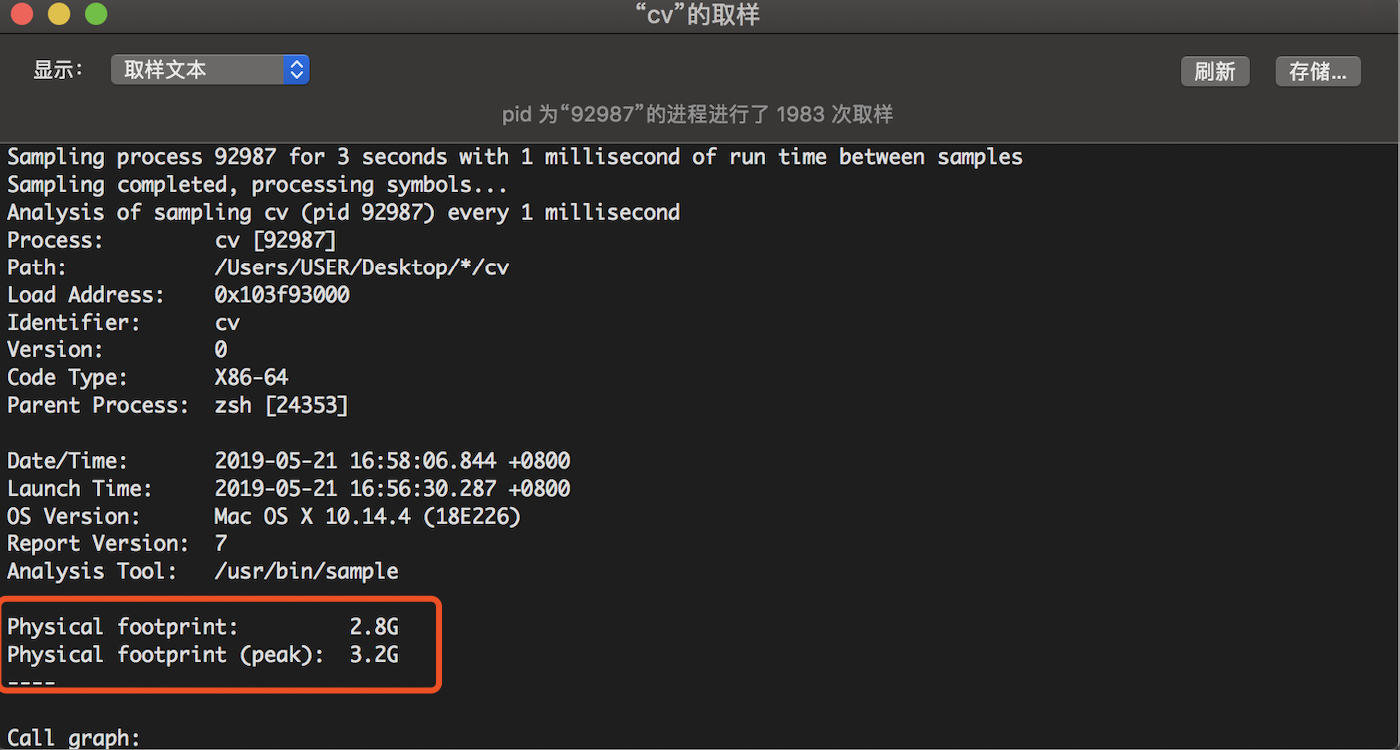
\includegraphics[scale=0.5]{single-tree-memory.png}
        \caption{单棵决策树训练内存占用}
        \label{}
    \end{figure}

    \item Gradient Boosting: 3.4G
    \begin{figure}[H]
        \centering
        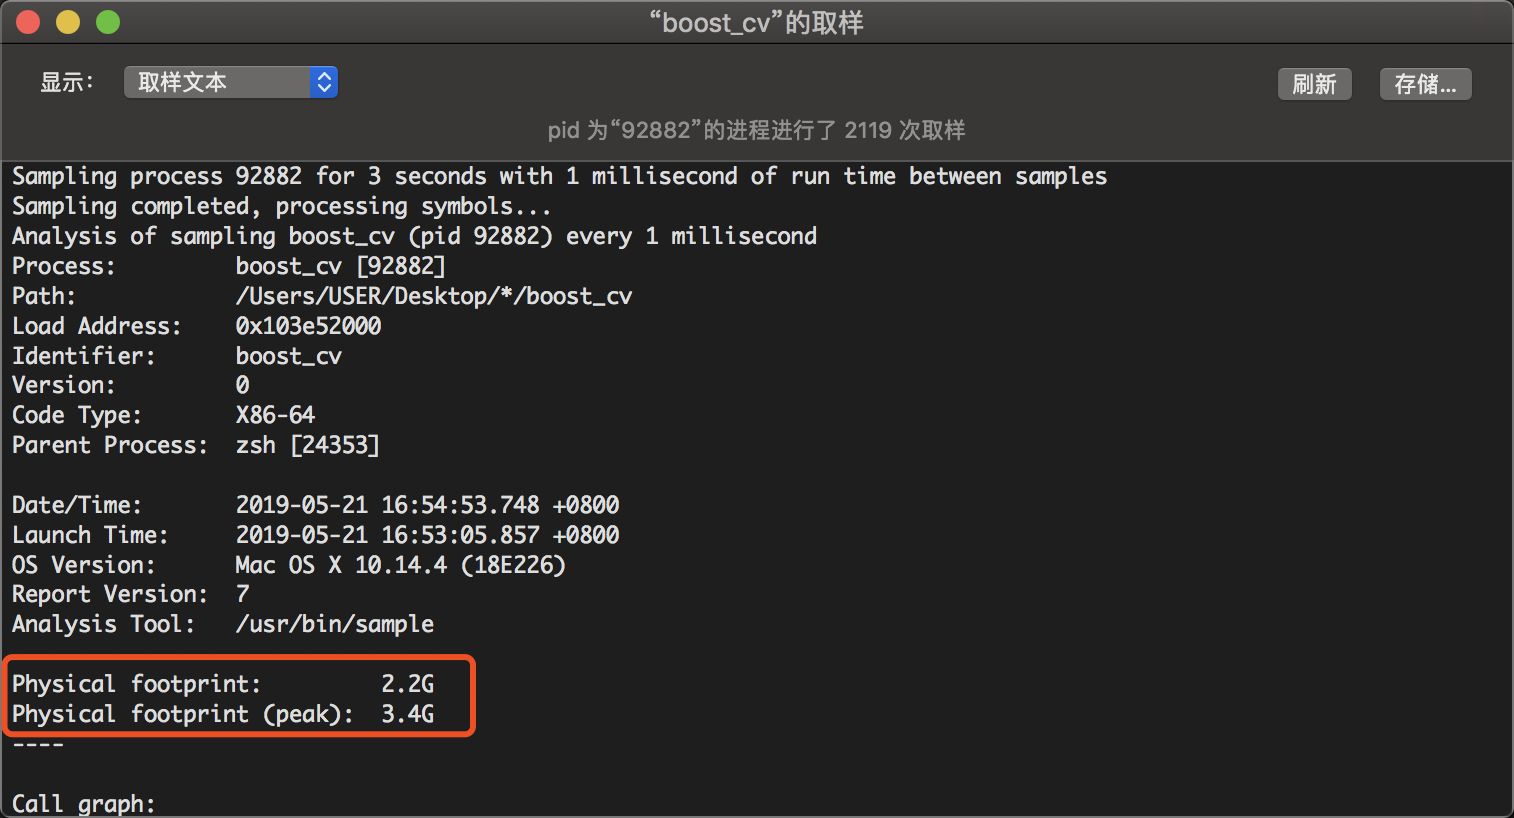
\includegraphics[scale=0.44]{gbdt-memory.png}
        \caption{Gradient Boosting训练内存占用}
        \label{}
    \end{figure}

    \item Random Forest: 1.6G
    \begin{figure}[H]
        \centering
        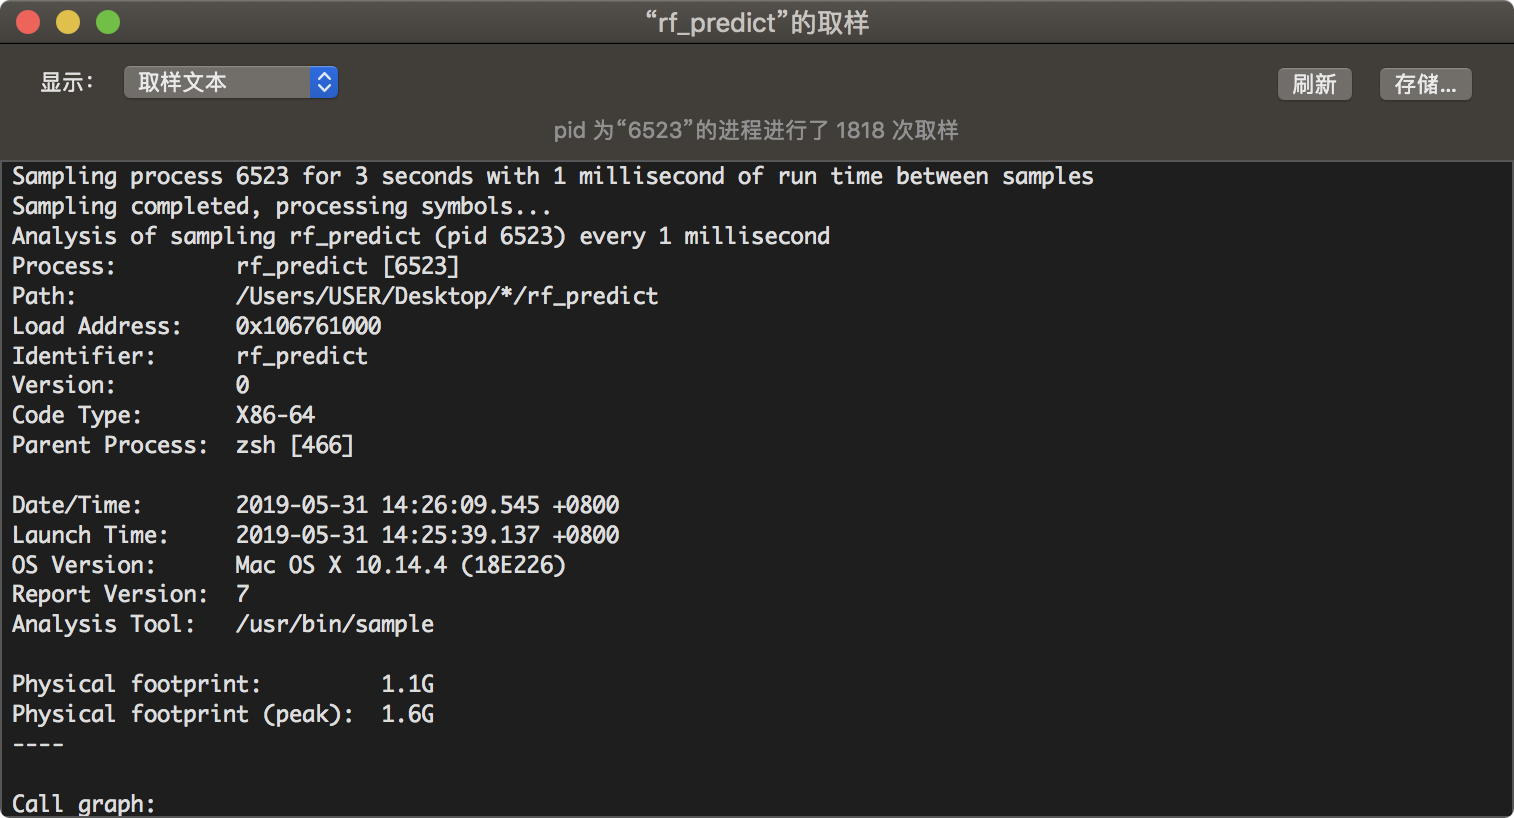
\includegraphics[scale=0.44]{rf-memory.png}
        \caption{Random Forest训练内存占用}
        \label{}
    \end{figure}
\end{enumerate}


\section{Kaggle 分数}

使用单棵决策树训练至10层后提交至 Kaggle 获得的分数为0.16087:
\begin{figure}[H]
    \centering
    
\includegraphics[scale=0.5]{single-tree-300-10-kaggle.png}
    \caption{单棵决策树分数}
    \label{}
\end{figure}

使用 Gradient Boosting, Learning Rate 固定为0.25,基学习器最大训练至3层,训练步数为400时的分数为0.16957:
\begin{figure}[H]
    \centering
    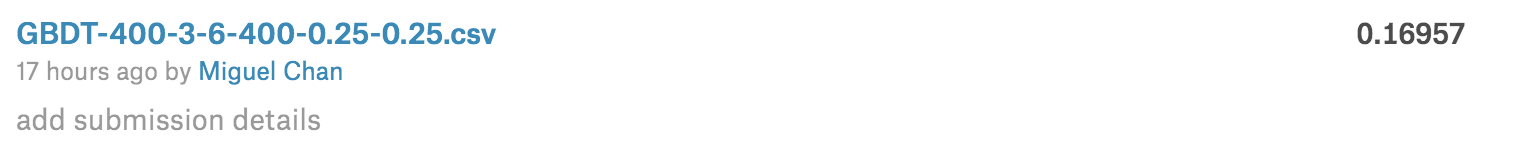
\includegraphics[scale=0.5]{gbdt-fixed-lr-kaggle.png}
    \caption{lr=0.25, GBDT}
    \label{}
\end{figure}

使用 Random Forest, 限制单棵决策树生长至10层,属性子集大小为3,\lstinline{SubSample}取0.632,分数为0.17433:
\begin{figure}[H]
    \centering
    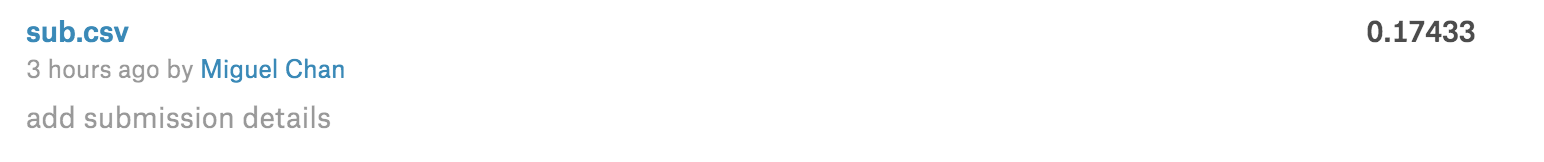
\includegraphics[scale=0.5]{best.png}
    \caption{随机森林}
    \label{}
\end{figure}

\bibliographystyle{unsrt}
\bibliography{ref}

\end{document}
\grid
\grid
